% Dies ist Teil der Vorlesung Physik auf dem Computer, SS 2012,
% Axel Arnold, Universitaet Stuttgart.
% 
% Dieses Werk ist unter einer Creative Commons-Lizenz vom Typ
% Namensnennung-Weitergabe unter gleichen Bedingungen 3.0 Deutschland
% zugänglich. Um eine Kopie dieser Lizenz einzusehen, konsultieren Sie
% http://creativecommons.org/licenses/by-sa/3.0/de/ oder wenden Sie sich
% schriftlich an Creative Commons, 444 Castro Street, Suite 900, Mountain
% View, California, 94041, USA.

\chapter{Numerisches Differenzieren und Integrieren}

In diesem Kapitel geht es darum, wie eine Funktion, die an diskreten
Stützstellen gegeben ist, numerisch differenziert und integriert
werden kann. Die Grundlagen dazu wurden bereits mit dem Kapitel
``Darstellung von Funktionen'' gelegt: für die numerische Ableitung
liegt es nahe, aus der Taylorentwicklung geeignete Ausdrücke für die
Ableitungen zu gewinnen, und für die Integration bieten sich das
interpolierende Polynom oder auch ein Spline and, die sich mit dem
Computer leicht analytisch integrieren lassen.

Numerisches Integrieren und Differenzieren kann dabei nicht nur dazu
dienen, Integrale oder Ableitungen abzuschätzen, sondern erlaubt auch,
einfache Differential- oder Integralgleichungen numerisch zu
lösen. Dazu muss die Gleichung mit Hilfe der hier vorgestellten
Verfahren diskretisiert und das resultierende lineare Gleichungssystem
gelöst werden.

\section{Numerisches Differenzieren}

Die erste Ableitung einer Funktion $f\in C^1([a,b])$ ist definiert als
\begin{equation}
  \lim_{h\to 0} \frac{f(x+h) - f(x)}{h}.
\end{equation}
Um den Grenzwert abzuschätzten, liegt es nahe, die Ableitung durch die
dividierte Differenz
\begin{equation}
  f'(\xi) \approx f[x,y] := \frac{f(x) - f(y)}{x - y}
\end{equation}
anzunähern, wobei $x$ und $y$ beide nahe bei $\xi$ liegen sollten.

Doch an welchem Punkt $\xi$ ist diese Näherung optimal? Gemäß
Mittelwertsatz gilt auf jeden Fall $f[x,y]=f'(\xi)$ für ein $\xi\in
[x,y]$. Man erwartet daher, dass $f[x,y]$ am besten in der
Intervalmitte $m=\frac{x+y}{2}$ approximiert. Das ist tatsächlich so,
wie wir nun per Taylorentwicklung sehen werden. Mit Entwicklung um $m$
und $h=x-y$ gilt
\begin{align}
  \frac{f(x) - f(y)}{x-y} &= \frac{1}{h}
  \biggl(+f(m) + \frac{h}{2}f'(m) + \frac{h^2}{8}f''(m) + \O(h^3)\nonumber\\
  &\phantom{= \frac{1}{h}\biggl(}-f(m) + \frac{h}{2}f'(m) - \frac{h^2}{8}f''(m) + \O(h^3)
  \biggr)\nonumber\\
  &=  f'(m) + \O(h^2).
\end{align}
Bei Ansatzpunkt $x$ gilt hingegen nur
\begin{align}
  \frac{f(x) - f(y)}{x-y} = \frac{1}{h}
  \biggl(f(x) + h f'(x) + \frac{h^2}{8}f''(x) + \O(h^3) - f(x) \biggr)
  =  f'(x) + \O(h).
\end{align}

In der Praxis ist die Funktion meist an an äquidistanten Stützstellen
$x_i$ mit $x_{i+1}-x_i=h$ gegeben. Dann ist, wie oben gezeigt, die
beste Zweipunkt-Näherung für die Ableitung die zentrale Differenz
\begin{equation}
  \label{eq:2orderdiff}
  \frac{f(x_{i+1}) - f(x_{i-1})}{2h} = f[x_{i-1},x_{i+1}] = f'(x_i) + \O(h^2),
\end{equation}
während für die linken und rechten dividierten Differenzen gilt:
\begin{equation}
  \frac{f(x_{i+1}) - f(x_{i})}{h} = f[x_{i},x_{i+1}] = f'(x_i) + \O(h)
\end{equation}
bzw.
\begin{equation}
  \frac{f(x_{i}) - f(x_{i-1})}{h} = f[x_{i},x_{i-1}] = f'(x_i) + \O(h).
\end{equation}

\subsection{Näherungen höhererer Ordnung und höhere Ableitungen}

Mit Hilfe von Taylorentwicklungen lassen sich auch Näherungen mit mehr
Stützpunkten und für höhere Ableitungen entwickeln.  Wir betrachten
zum Beispiel die Punkte für $k=-2(1)2$, d.h. die 5 benachbarten
Punkte, und suchen Koeffizienten $c_k$ derart, dass
\begin{equation}
  c_2 f(x_{i+2}) + c_1 f(x_{i+1})  + c_0 f(x_i) + c_{-1}f(x_{i-1}) +
  c_{-2}f(x_{i-2}) = f'(x_i) + \O(h^5),
\end{equation}
unabhänging von der Form von $f$ und seiner Ableitungen.  Durch
Einsetzen der Taylorentwicklung
\begin{equation}
  f(x + k h) = f(x) + k\, hf'(x) + k^2\,\frac{h^2}{2} f''(x_i) +
  k^3\,\frac{h^3}{6}f^{(3)}(x) + k^4\,\frac{h^4}{24}f^{(4)}(x) + \O(h^5)
\end{equation}
folgt dann, in der Reihenfolge der Ableitungen in der Taylorentwicklung
\begin{align}
  \label{eq:derivatives}
  c_{2} + c_{-2} + c_{-1} + c_1 + c_0 &= 0\nonumber\\
  h\left[2 (c_{2} - c_{-2})  + c_{1} - c_{-1}\right] &= 1\nonumber\\
  \frac{h^2}{2}\left[4(c_{2} + c_{-2})  + c_{1} + c_{-1}\right] &= 0\nonumber\\
  \frac{h^3}{6}\left[8 (c_{2} - c_{-2})  + c_{1} - c_{-1}\right] &= 0\nonumber\\
  \frac{h^4}{24}\left[16 (c_{2} + c_{-2}) + c_{1} + c_{-1}\right] &= 0.
\end{align}
Durch Lösen des Gleichungssystems folgt
\begin{equation}
  \label{eq:4orderdiff}
  -\frac{1}{12h} f(x_{i+2}) + \frac{2}{3h} f(x_{i+1})  - \frac{2}{3h} f(x_{i-1}) +
  \frac{1}{12h}f(x_{i-2}) = f'(x_i) + \O(h^4).
\end{equation}
Auf diese Weise lässt sich auch die höhere Güte der zentralen
Differenz verstehen: tatsächlich entspricht diese der optimalen
Näherung durch $x_{i-1}$, $x_i$  und $x_{i+1}$, nur dass aus
Symmetriegründen der Koeffizient zu $x_i$ verschwindet.

Um nun zum Beispiel die zweite Ableitung zu berechnen, lösen wir
\eqref{eq:derivatives}, allerdings mit einer 1 nicht in der zweiten,
sondern dritten Zeile. Das ergibt
\begin{equation}
  \label{eq:3order2diff}
  \frac{1}{h^2}\left(-\frac{1}{12} f(x_{i+2}) + \frac{4}{3} f(x_{i+1}) +
  \frac{5}{2} f(x_i)  + \frac{4}{3} f(x_{i-1}) -
  \frac{1}{12}f(x_{i-2})\right) = f''(x_i) + \O(h^3).
\end{equation}

Mit drei Stützpunkten ergibt sich die Näherung für die zweite
Ableitung analog als
\begin{multline}
  \label{eq:1order2diff}
  \frac{1}{h^2}\bigl(f(x_{i+1}) -
  2f(x_i)  + f(x_{i-1})\bigr) =
  \frac{\frac{f(x_{i+1}) - f(x_i)}{h}  -
    \frac{f(x_i) - f(x_{i-1})}{h}}{h}
  = f''(x_i) + \O(h).
\end{multline}
Die mittlere Form zeigt, dass sich diese einfachste Form der zweiten
Ableitung auch als dividierte Differenz der dividierten Differenzen
verstehen lässt. Technisch wird also die zweite Ableitung also einfach
in erster Ordnung aus der ersten Ableitung in erster Ordnung
bestimmt. Analog lässt sich jede $n$-te Ableitung aus $n+1$
benachbarten Stützstellen in erster Ordnung durch dividierte
Differenzen approximieren.

\begin{figure}
  \centering
  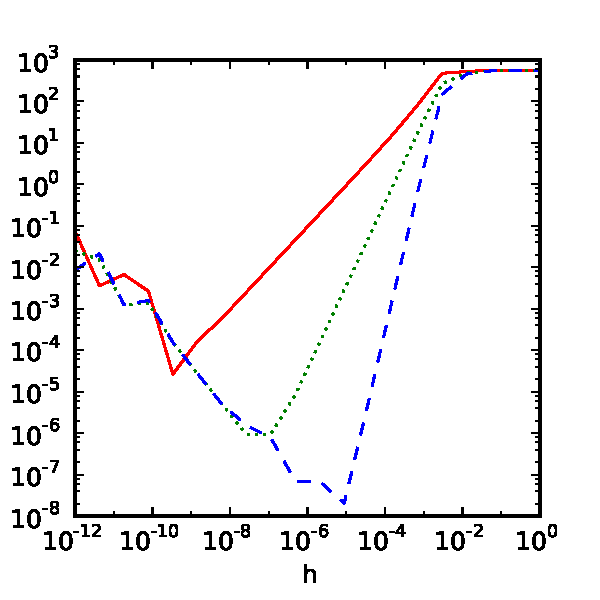
\includegraphics[width=0.5\textwidth]{plots/num_diff}
  \caption{Maximale Abweichung $\max_{x\in[-\pi,pi]} \abs{f'(x) - a(h;
      x)}$ für verschiedene Näherungen $a(h; x)$, als Funktion der
    Schrittweite $h$. Die Funktion ist $f(x)=sin(100x^2)$. Rot
    durchgezogen ist die linksseitige Differenz $a(h; x) = (f(x) -
    f(x-h))/h$, die zentrale Differenz $a(h; x) = (f(x+h) -
    f(x-h))/2h$ ist grün gepunktet und die Näherung 4. Ordnung
    \eqref{eq:4orderdiff} blau gestrichelt. Der rechtsseitige Abfall
    der Kurven entspricht den Ordnungen $\O(h)$ für die linksseitige
    Differenz, $\O(h^2)$ für die rechtsseitige und $\O(h^4)$ für die
    Gleichung 4. Ordnung. Das linksseitige Verhalten ist
    methodenunabhängig und durch die endliche Rechenauflösung bestimmt.}
  \label{fig:num_diff}
\end{figure}

\subsection{Genauigkeit}

Generell sind alle diese Näherungen numerisch instabil, da bei kleinen
Abständen $h$ auch $f(x)$ und $f(x+h)$ sehr ähnlich sind. Sind diese
betragsmäßig groß, kommt es zu Auslöschung, d.h., $f(x+h) - f(x)$ hat
deutlich weniger signifikante Stellen als Maschinengenauigkeit. Daher
gibt es stets ein optimales $h$, das allerdings von der unbekannten
zweiten Ableitung der betrachteten Funktion abhängt.

Auch Verfahren höherer Ordnung sind nicht notwendigerweise genauer, da
bei manchen Funktionen die Ableitungen sehr rasch wachsen. Dann ist
zwar $h^4$ sehr viel kleiner als $h^2$, aber der Vorfaktor
kompensiert das zunächst. Abbildung~\ref{fig:num_diff} illustriert
dieses Verhalten am Beispiel der Funktion $\sin(100x^2)$. Erst, wenn
die Schrittweite $h$ unter die charakteristische Breite von etwa 600
sinkt, spielt die Ordnung des Verfahrens eine Rolle. Wird allerdings
$h$ zu klein, zeigt sich die endliche Auflösung, mit der der Rechner
arbeitet, und der Fehler steigt wieder an.

\subsection{Beispiel}

Wir betrachten die Besselsche Differentialgleichung, eine gewöhnliche
lineare Differentialgleichung zweiter Ordnung:
\begin{equation}
  \label{eq:besselode}
  x^2\frac{d^2f}{dx^2} + x\frac{df}{dx} + (x^2-\nu)f = 0
\end{equation}
für $f\in C^{\infty}([0,\infty))$. Die Besselsche
Differentialgleichung spielt eine wichtige Rolle in der Physik, weil
sie den radialen Anteil der Laplacegleichung in Zylinderkoordinaten
beschreibt.  Für die Lösungen dieser Gleichung lassen sich schnell
konvergierende Reihen oder Integraldarstellungen
angeben~\cite{abramowitz70a,jackson99}, wir wollen aber zu
Demonstrationszwecken diese Differentialgleichung für $\nu=0$
numerisch lösen. Hierzu definieren wir $f_k := f(kh)$, $k\ge 0$, und
diskretisieren \eqref{eq:besselode} mit Hilfe der finiten Differenzen
\eqref{eq:2orderdiff} und \eqref{eq:1order2diff} in linearer Ordnung:
\begin{align}
  \label{eq:besseldiscrete}
  0 &= k^2\left(\frac{1}{2} f_{k-1} - f_k + \frac{1}{2} f_{k+1} \right)
  + k\left(\frac{1}{2} f_{k+1} - \frac{1}{2} f_{k-1}\right)
  + k^2h^2f_k\nonumber\\
  &= \frac{1}{2}(k^2 - k)f_{k-1}
  + k^2(h^2 - 1)f_k
  + \frac{1}{2}(k^2 + k)f_{k+1}.
\end{align}
Für die Lösung $f$ auf dem endlichen Interval $[0, (N-1)h]$ sind das
$N-2$ Gleichungen, da für die Randpunkte die zweite Ableitung so nicht
abgeschätzt werden kann. Dies ist aber auch nicht weiter
verwunderlich, da wir ja die Randbedingungen noch nicht festgelegt
haben. Die natürlichen Randbedingungen der Diskretisierung sind also
Dirichlet-Randbedingungen, bei denen die fehlenden Randwerte
vorgegeben werden.

$f_0$ erscheint allerdings in keiner weiteren Gleichung gemäß
\eqref{eq:besseldiscrete}, da $k^2-k=0$ für $k=1$. Wird also $f_0$
vorgegeben, so ist der Verlauf der Gleichung im Bereich $\ge h$ nur
durch den rechten Rand (unter-)bestimmt. Dies deutet bereits an, dass
diese einfachste Disretisierung der Gleichung problematisch sein
könnte. Man kann nun versuchen, dass Problem zu umgehen, in dem $f$
stattdessen im Bereich $[h, Nh]$ betrachtet wird. Wir erhalten das
folgende lineare Gleichungssystem:
\begin{equation}
  \begin{pmatrix}
    1 & 0         & 0         &\ldots & \ldots & 0\\
    1 & -4\lambda & 3         & 0 & \ldots & 0\\
    0 & 3         & -9\lambda & 6 & 0\quad \ldots & 0\\
    & & \ddots & \ddots & \ddots\qquad\qquad \\
    0 & \ldots & 0 & \frac{1}{2}(N-1)(N-2) & -(N-1)^2\lambda & \frac{1}{2}(N^2-N)\\
    0 &          &  \ldots  &   & 0      & 1
  \end{pmatrix}
  \begin{pmatrix}
    f_1\\
    \vdots\\
    f_N
  \end{pmatrix}=
  \begin{pmatrix}
    F_1\\
    0\\
    0\\
    \vdots\\
    0 \\
    F_N
  \end{pmatrix},
\end{equation}
wobei $\lambda=(1-h^2)$. Die beiden äußeren Zeilen implementieren die
Dirichletbedingungen $f_1 = f(h)=F_1$ und $f_N = f(Nh) = F_n$, die
restlichen $N-2$ Zeilen Gleichung \eqref{eq:besseldiscrete} für
$k=2(1)N$.  Da die Matrix Bandstruktur hat, können wir dieses lineare
Gleichungssystem effizient mit dem Gaußverfahren lösen.

\begin{figure}
  \centering
  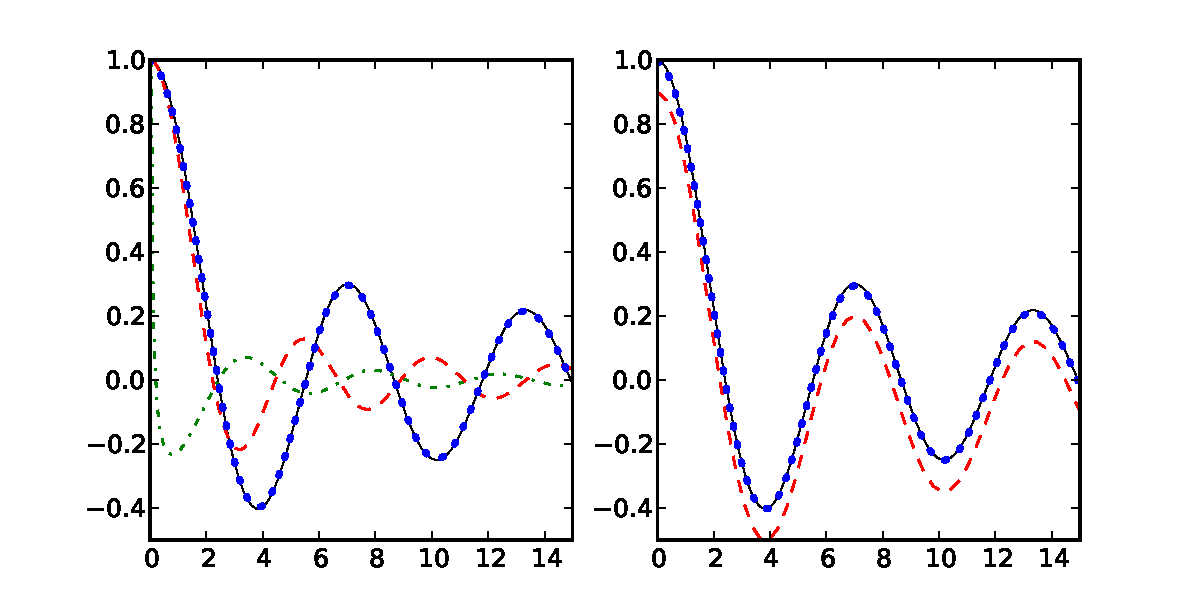
\includegraphics[width=\textwidth]{plots/bessel}
  \caption{Links: numerische Lösungen der Besselschen
    Differentialgleichung mit Schrittweite $h=0,05$. Die durchgezogene
    schwarze Linie markiert die analytische Lösung. Mit grünen
    Strichpunkten ist die Lösung mit Hilfe von
    \eqref{eq:besseldiscrete} und Dirichletrandbedingungen im Bereich
    $[h, 15]$ dargestellt, rot gestrichelt mit Vorgabe von
    Funktionswert und Ableitung bei $h$. Blaue Punkte schliesslich
    markieren den Löser dritter Ordnung mit Dirichletrandbedingungen,
    der von der analytischen Lösung nicht zu unterscheiden
    ist. Rechts: numerische Lösung des Besselintegrals mit 300 (blaue
    Punkte) und 10 Stützpunkten (rot gestrichelt) im Interval
    $[0,\pi]$.}
  \label{fig:bessel}
\end{figure}

Die Lösung dieses Gleichungssystems ist in Abbildung~\ref{fig:bessel}
mit grünen Strichpunkten gezeigt. Sie hat allerdings wenig mit der
korrekten Lösung gemeinsam. Der tiefere Grund ist, dass die Besselsche
Differentialgleichung für ganzzahlige $\nu$ nicht nur die in $0$
beschränkte Lösung hat, die wir suchen, sondern auch eine
unbeschränkte. Da wir aber in linearer Ordnung keine Gleichung
erhalten, die den Punkt 0 mit den restlichen Punkten verbindet, kann
die Lösung im Bereich $>h$ prinzipiell auch zur singulären Lösung
gehören und daher eine sehr steile Ableitung aufweisen, wie eben
unsere Lösung.

Um dieses Problem zu umgehen, könnte man nun statt der Randwerte den
Funktionswert und die erste Ableitung am linken Rand vorschreiben,
also $F_1 = f(h) = f_h$ und $ F'_1 = \nicefrac{d}{dx}f(h) \approx
\frac{1}{h} f_{2h} - \frac{1}{h}f_h$.  Wie Abbildung~\ref{fig:bessel}
in rot gestrichelt zeigt, ist dann die Lösung am linken Rand
tatsächlich besser, aber am rechten Rand immer noch nicht
befriedigend. Auch durch Verringern der Schrittweite $h$ verbessert
sich die Lösung nicht deutlich.

Abhilfe schafft, auf Verfahren höherer Ordnung zurückzugreifen, etwa
\eqref{eq:3order2diff} und \eqref{eq:4orderdiff}. In dieser Ordnung
taucht $f_0$ in der Hauptgleichung
\begin{align}
  0 = &\frac{1}{12}(-k^2 + k)f_{k-2}
  + \frac{2}{3}(2k^2 - k)f_{k-1}
  + k^2\left(h^2 - \frac{5}{2}\right)f_k\nonumber\\
  &+ \frac{2}{3}(2k^2 - k)f_{k+1}
  + \frac{1}{12}(-k^2 + k)f_{k+2}
\end{align}
auch für $k=2$ auf. Durch den breiteren Rand benötigt diese Gleichung
ingesamt vier Startwerte. Von diesen benutzen wir zwei als
Dirichletbedingungen $f_0 = F_0$ und $f_{N-1} = F_{N-1}$, und
generieren daraus über Gleichung \eqref{eq:besseldiscrete} Näherungen
für $f_1$ und $f_{N-2}$. Die Lösung dieses Gleichungssystem ist in
Abbildung~\ref{fig:bessel} blau gepunktet eingezeichnet und nicht mehr
von der analytischen Lösung zu unterscheiden. Dies zeigt den Nutzen
von Ableitungsnäherungen höherer Ordnung.

\section{\keyword{Quadratur}: \keyword{numerische Integration}}

Bei der numerischen Integration geht es genau wie beim Differenzieren
darum, aus endlich vielen Stützwerten das Integral einer Funktion in
einem endlichen Interval abzuschätzen. Wir suchen also Gewichte
$\alpha_{i}\in\RR$, so dass möglichst genau
\begin{equation}
  \int_a^b f(x)\, dx \approx \sum_{i=0}^{n-1} \alpha_if(x_i),
\end{equation}
wobei die $\alpha_i$ von der Lage der Stützpunkte ("`Knoten"') $x_i$
abhängen, aber nicht von $f$. Dadurch, dass die Funktion über dem
ganzen Interval $[a,b]$ in das Integral eingeht, wird man für die
numerische Integration natürlich mehr Punkte als beim Differenzieren
einbeziehen wollen, und hat dementsprechend auch mehr Möglichkeiten,
die Gewichte zu wählen. Im folgenden werden wir einige der
gebräuchlichsten Verfahren kennenlernen.

\subsection{\keyword{Newton-Cotes-Formeln}}

Um eine an diskreten Stützstellen $x_i$, $i=0(1)n-1$ gegebene Funktion
$f$ zu integrieren, liegt es nahe, die Funktion mit Hilfe eines
Polynoms zu interpolieren und dieses dann analytisch zu integrieren:
\begin{equation}
  \int_a^b f(x)\, dx \approx
  \int_a^b \sum_{i=0}^{n-1} f(x_i) L_i(x) \, dx = \sum_{i=0}^{n-1}
  \underbrace{\int_a^b
  L_i(x) dx}_{\alpha_i}\, f(x_i).
\end{equation}
Diese \emph{Newton-Cotes-Formeln} integrieren offenbar alle Polynome
bis Ordnung $n$ exakt. Allerdings verstärkt sich bei allgemeinen
Funktion das Rungephänomen bei der Integration, und ab Ordnung $n=9$
treten negative Koeffizienten $\alpha_i$ auf, was die Näherung
verschlechtert. Daher sind nur kleine $n$ sinnvoll, und in der Praxis
werden meist nur Formeln bis Ordnung $n=8$ benutzt. Die
gebräuchlichsten sind in Abbildung~\ref{fig:intregel} skizziert und
werden im folgenden kurz diskutiert.

\begin{figure}
  \centering
  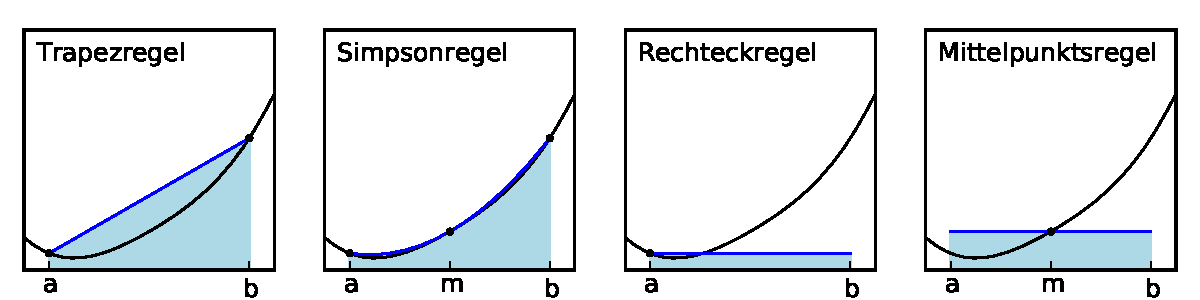
\includegraphics[width=\textwidth]{plots/num_int}
  \caption{Illustration der vier Newton-Cotes-Formeln. Die Punkte
    markieren die Stützpunkte, hellblau ist die Fläche unter dem
    interpolierenden Polynom, die der Näherung des Integrals dient.}
  \label{fig:intregel}
\end{figure}
\subsubsection{\keyword{Trapezregel}}

Die Trapezregel benutzt als Stützstellen $x_0=a$ und $x_1=b$:
\begin{equation}
  \int_a^b f(x)\, dx \approx f(a)\int_a^b \frac{x-b}{a-b}\,dx \,+\,
  f(b)\int_a^b \frac{x-a}{b-a}\,dx
  \,=\, \frac{b-a}{2} \Bigl(f(a) + f(b)\Bigr).
\end{equation}
Weiter gilt
\begin{multline}
  \int_a^b f(x)\, dx - \frac{b-a}{2} \Bigl(f(a) + f(b)\Bigr)
  =  \int_a^b f(x) - f(a)\frac{x-b}{a-b}
  + f(b)\frac{x-a}{a-b}\, dx\\
  =  \int_a^b
  {}\bigl(f(x) - f(a)\bigr)\frac{x-b}{a-b}
  + \bigl(f(b) - f(x)\bigr)\frac{x-a}{a-b}\, dx\\
  =  \int_a^b
  \frac{1}{a-b}\left(\frac{f(x) - f(a)}{x-a} + \frac{f(b) - f(x)}{x-b}\right)
  \underbrace{(x-b)(x-a)}_{<0 \text{ in } [a,b]}\, dx\\
  =
  \frac{f''(\xi)}{2}\int_a^b (x-b)(x-a)\, dx = \frac{(b-a)^3}{12} f''(\xi)
\end{multline}
für ein $\xi\in[a,b]$. Gibt es also eine Abschätzung für die zweite
Ableitung von $f$, so lässt sich auch der Fehler der Trapezregel
abschätzen. Ist $f$ konvex auf $[a,b]$, also $f''(\xi)>0$, so
unterschätzt also die Trapezregel das Integral, ist $f$ konkav,
überschätzt sie es.

\subsubsection{Simpsonregel}

Analog wird die Simpsonregel für die drei Stützpunkte $x_0=a$,
$x_1=\frac{a+b}{2}$ und $x_2=b$ definiert:
\begin{equation}
  \int_a^b f(x)\, dx = \frac{b-a}{3} \left(f(a) +
  4 f\left(\frac{a+b}{2}\right) + f(b)\right) +
  \frac{(b-a)^5}{90} f^{(4)}(\xi)
\end{equation}
für ein $\xi\in[a,b]$.

\index{Newton-Cotes-Formeln>offene}
\index{Newton-Cotes-Formeln>geschlossene}

Die Simpsonregel und die Trapezregel sind die meistgenutzten
\emph{geschlossenen} Newton-Cotes-Formeln. Geschlossen heißen solche
Formeln, die $a$ und $b$ als Stützpunkte beinhalten. \emph{Offene}
Formeln dagegen enthalten wenigstens einen der Punkte
nicht. Naturgemäß sind die beiden folgenden Einpunktformeln offen.

\subsubsection{Rechteckregel}

Wir benutzen $x_0=a$ als Stützpunkt, und erhalten:
\begin{equation}
  \int_a^b f(x)\, dx = (b-a) f(a) +
  \frac{(b-a)}{2} f'(\xi)
\end{equation}
für ein $\xi\in[a,b]$.

\subsubsection{Mittelpunktsregel}

Wir benutzen $x_0=\frac{a+b}{2}$ als Stützpunkt, und erhalten:
\begin{equation}
  \int_a^b f(x)\, dx = (b-a) f(\frac{a+b}{2}) +
  \frac{(b-a)^3}{24} f''(\xi)
\end{equation}
für ein $\xi\in[a,b]$. Ähnlich wie schon beim Differenzieren ist also
der Intervallmittelpunkt ausgezeichnet.

\subsection{Zusammengesetzte Quadraturregeln}


\subsection{Richardson-Extrapolation}
Romberg-Verfahren

\subsection{Gauß-Quadratur}

\subsection{Unbegrenzte Intervalle und Singularitäten}

\subsection{Monte-Carlo-Integration}
Curse of dimension

\subsubsection{Beispiel: Berechung von $\pi$}



%%% Local Variables: 
%%% mode: latex
%%% TeX-master: "padc.tex"
%%% TeX-PDF-mode: t
%%% End: 
